%


\documentclass[twoside]{article}
\setlength{\oddsidemargin}{0.25 in}
\setlength{\evensidemargin}{-0.25 in}
\setlength{\topmargin}{-0.6 in}
\setlength{\textwidth}{6.5 in}
\setlength{\textheight}{8.5 in}
\setlength{\headsep}{0.75 in}
\setlength{\parindent}{0 in}
\setlength{\parskip}{0.1 in}

%
% ADD PACKAGES here:
%

\usepackage{amsmath,amsfonts,graphicx}

%
\newcounter{lecnum}
\renewcommand{\thepage}{\thelecnum-\arabic{page}}
\renewcommand{\thesection}{\thelecnum.\arabic{section}}
\renewcommand{\theequation}{\thelecnum.\arabic{equation}}
\renewcommand{\thefigure}{\thelecnum.\arabic{figure}}
\renewcommand{\thetable}{\thelecnum.\arabic{table}}

%
% The following macro is used to generate the header.
%
\newcommand{\lecture}[4]{
   \pagestyle{myheadings}
   \thispagestyle{plain}
   \newpage
   \setcounter{lecnum}{#1}
   \setcounter{page}{1}
   \noindent
   \begin{center}
   \framebox{
      \vbox{\vspace{2mm}
    \hbox to 6.28in { {\bf EE302 - Feedback Systems
	\hfill Spring 2019} }
       \vspace{4mm}
       \hbox to 6.28in { {\Large \hfill Lecture #1 \hfill} }
       \vspace{2mm}
       \hbox to 6.28in { {\it Lecturer: #2 \hfill } }
      \vspace{2mm}}
   }
   \end{center}
   \markboth{Lecture #1}{Lecture #1}

   \vspace*{4mm}
}
%
\renewcommand{\cite}[1]{[#1]}
\def\beginrefs{\begin{list}%
        {[\arabic{equation}]}{\usecounter{equation}
         \setlength{\leftmargin}{2.0truecm}\setlength{\labelsep}{0.4truecm}%
         \setlength{\labelwidth}{1.6truecm}}}
\def\endrefs{\end{list}}
\def\bibentry#1{\item[\hbox{[#1]}]}

%Use this command for a figure; it puts a figure in wherever you want it.
%usage: \fig{NUMBER}{SPACE-IN-INCHES}{CAPTION}
\newcommand{\fig}[3]{
			\vspace{#2}
			\begin{center}
			Figure \thelecnum.#1:~#3
			\end{center}
	}
% Use these for theorems, lemmas, proofs, etc.
\newtheorem{theorem}{Theorem}[lecnum]
\newtheorem{lemma}[theorem]{Lemma}
\newtheorem{proposition}[theorem]{Proposition}
\newtheorem{claim}[theorem]{Claim}
\newtheorem{corollary}[theorem]{Corollary}
\newtheorem{definition}[theorem]{Definition}
\newenvironment{proof}{{\bf Proof:}}{\hfill\rule{2mm}{2mm}}

% **** IF YOU WANT TO DEFINE ADDITIONAL MACROS FOR YOURSELF, PUT THEM HERE:

\begin{document}

% Lecture Details
\lecture{16}{Asst. Prof. M. Mert Ankarali}

\par

\section{Nyquist Stability Criterion for Feedback Systems}

Even though we illustrated how to apply Nyquist stability criterion
for feedforward systems in the previous lecture (for teaching the
details of Nyquost plot and some basics), in control theory and
applications Nyqist plot and Nyquist stability test are majorly used for
analyzing feedback topologies. 

\subsection{Nyquist Stability for Feedback Systems}

The figure below illustrates the fundamental feedback system topology for a SISO system

\vspace{6 pt}

  \begin{minipage}[h]{1\linewidth}
    \begin{center}
      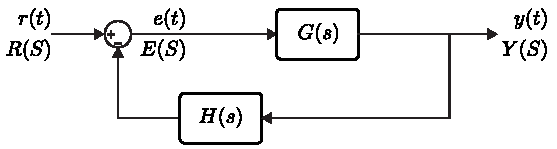
\includegraphics[width=0.5\textwidth]{unityfeedback}
    \end{center}
  \end{minipage}

\vspace{6 pt}

We know that the closed-loop transfer function, $T(s)$, for this
system has the following form
%
\begin{align*}
  T(s) = \frac{G(s)}{1 + G(s) H(s)} = \frac{G(s)}{1 + G_{OL}(s)}  
\end{align*}
%
where $G_{OL}(s)$ is the open-loop transfer function for the given
topology. We know that poles of $T(s)$ are the roots that satisfy 
$1 + G_{OL}(s) = 0$. Now let's define an analytic function $F(s) = 1 +
G_{OL}(s)$, analyze its relation with the open-loop and closed-loop
transfer functions. 
%
\begin{align*}
  F(s) = 1 + G_{OL}(s) = 1 + \frac{ N(s) }{ D(s) } = \frac{ D(s) + N(s) }{D(s)}
\end{align*}
%
where 
 %
\begin{itemize}
  \item Roots of $N(s)$ are open-loop zeros
  \item Roots of $D(s)$ are open-loop poles
\end{itemize}
%
Moreover 
 %
\begin{itemize}
  \item \textbf{Poles} of $F(s)$ are the roots of $D(s)$, hence they
    constitutes the \textbf{open-loop poles}.
  \item \textbf{Zeros} of $F(s)$ are the poles of $T(s)$, hence 
    they constitutes the \textbf{closed-loop poles}.
\end{itemize}
%
Note that open-loop zeros and poles are ``known'', and goal is 
to investigate/analyze the number of unstable poles of $T(s)$
which is equal to the number of zeros of $F(s)$ with positive real parts

Now let's assume that we derive Nyquist plots of $F(s) = 1 +
G_{OL}(s)$ and $G_{OL}(s)$ and obtain $\Gamma_{F(s)}$ and
$\Gamma_{G_{OL}(s)}$. The figure below provides an illustrative
example of a Nyquist contour, Nyquist plot of $F(s)$, and
Nyquist plot of $G_{OL}(s)$. 

\vspace{6 pt}

  \begin{minipage}[h]{1\linewidth}
    \begin{center}
      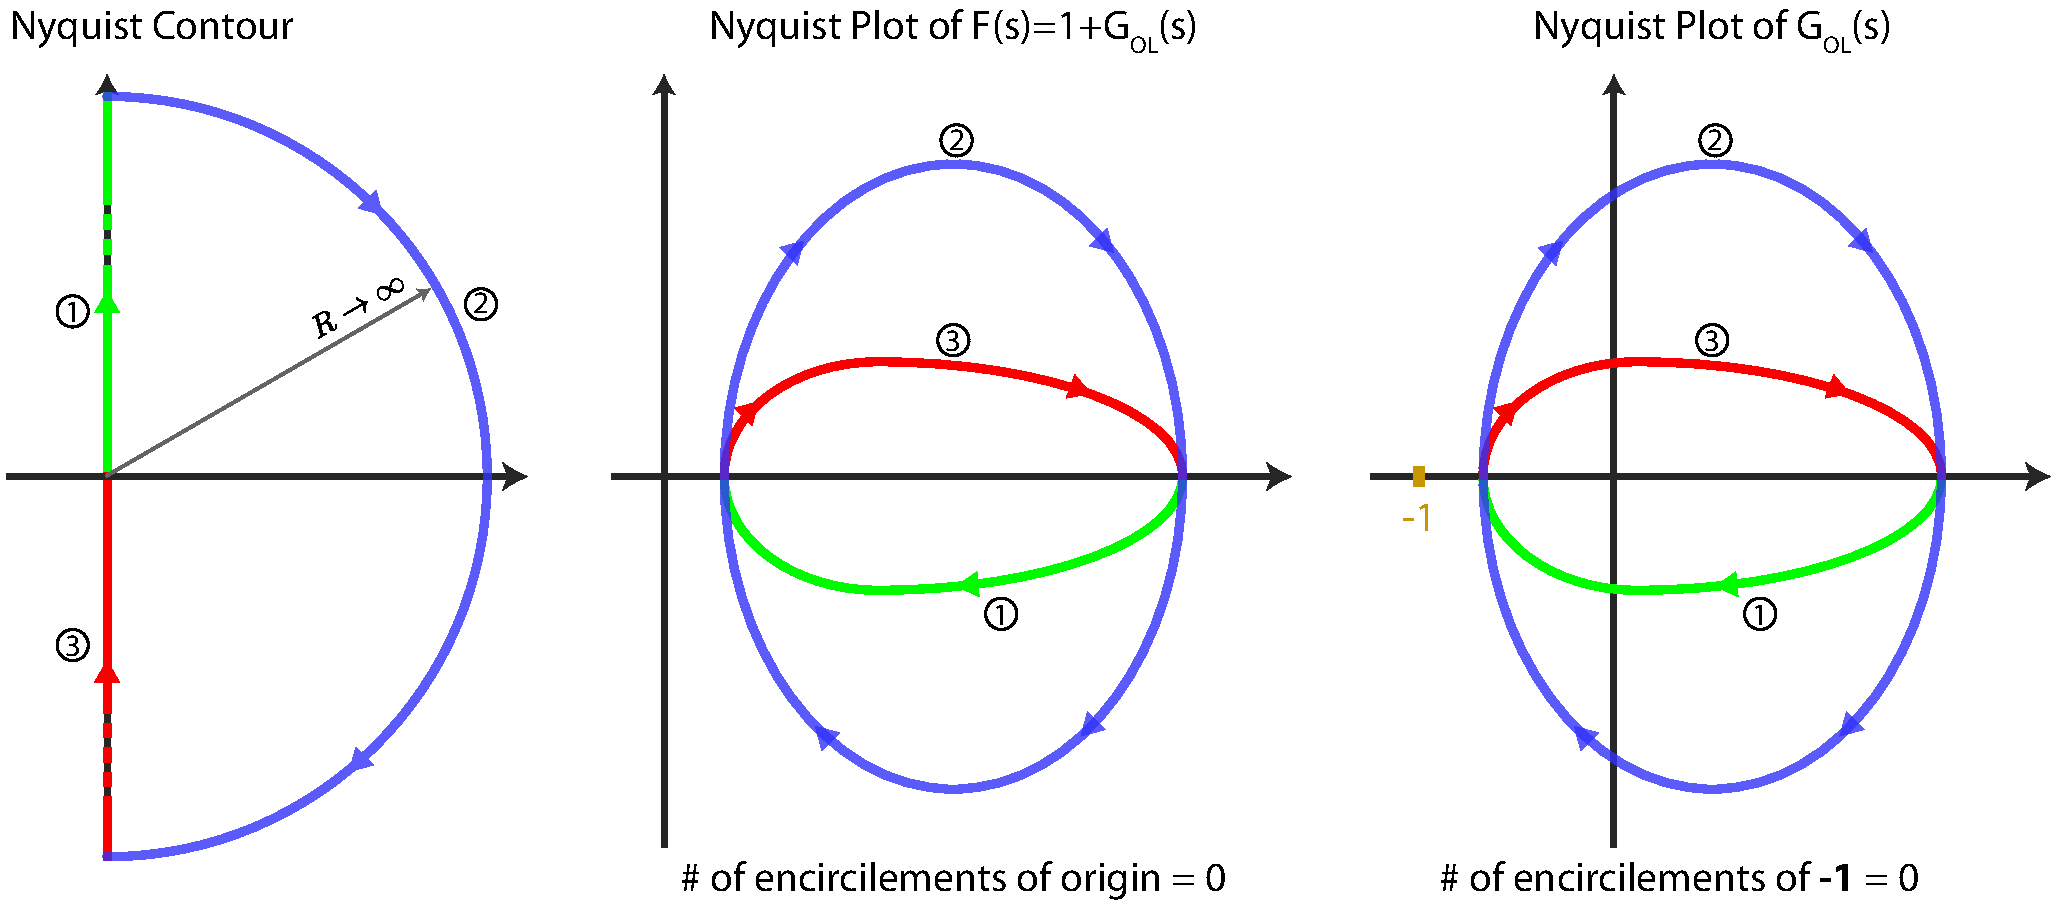
\includegraphics[width=0.9\textwidth]{nyq}
    \end{center}
  \end{minipage}

\vspace{6 pt}

First simple observation that we have to pay attention is that in order to obtain $\Gamma_{G_{OL}(s)}$ we
shift $\Gamma_{F(s)}$ on real axis to the left (by \textbf{1}), similarly  in order to obtain $\Gamma_{F(s)}$ we
shift $\Gamma_{G_{OL}(s)}$ on real axis to the right ((by
\textbf{1})). From this fact we can derive the following equality
which is critical for stability analysis

\vspace{6 pt}

N $\ = \ $ $\#$ of CW enrichments of origin by  $\Gamma_{F(s)}$ $ \ =\ $ $\#$ of
CW enrichments of $(-1 + 0 j)$ by  $\Gamma_{G_{OL}(s)}$. 

\vspace{6 pt}

For example In this illustration above $N =0$. If we apply
Cauchy's Principle argument for $F(s)$, we can derive that
%
\begin{itemize}
  \item $N = Z_F - P_F$ 
%
  \item $P_{F}$ : $\#$ poles of $F(s)$ with positive real parts, which is
    indeed equal to the $\#$ poles of $G_{OL}(s)$ with positive real
    parts which is a ``known'' quantity. 
%
  \item $Z_F$ : $\#$ zeros of $F(s)$ with positive real parts, which is
    indeed equal to to the $\#$ unstable poles of $T(s)$ which is the
   desired output.
\end{itemize}

In conclusion, in order to analyze the closed-loop stability of a 
unity-feedback feed-back systems we apply the following 
procedure 

\begin{itemize}
 \item Draw the Nyquist plot of $G_{OL}(s)$
 \item Compute $N = \ \#$ CW encirclements of $(-1 + 0 j)$ by
   $\Gamma_{G_{OL}(s)}$ 
 \item Compute $P_{F} = P_{OL} = \ \#$ open-loop poles with
   positive real parts
 \item Finally compute $\mathbf{P_{CL}} = Z_{F} = N +  P_F = \mathbf{N +  P_{OL}} = \ \#$
   unstable closed-loop poles  
\end{itemize}

\newpage

\textbf{Ex:} Analyze the stability of the following feedback system
using Nyquist plot.

\vspace{6 pt}

  \begin{minipage}[h]{1\linewidth}
    \begin{center}
      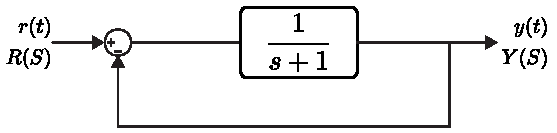
\includegraphics[width=0.5\textwidth]{ex1block}
    \end{center}
  \end{minipage}

\vspace{6 pt}

\textbf{Solution:} For this given system $G_{OL}(s) = \frac{1}{s+1}$.
In the previous lecture we already derived the Nyquist plot for $\frac{1}{s+1}$
which is illustrated below

\vspace{6 pt}

  \begin{minipage}[h]{1\linewidth}
    \begin{center}
      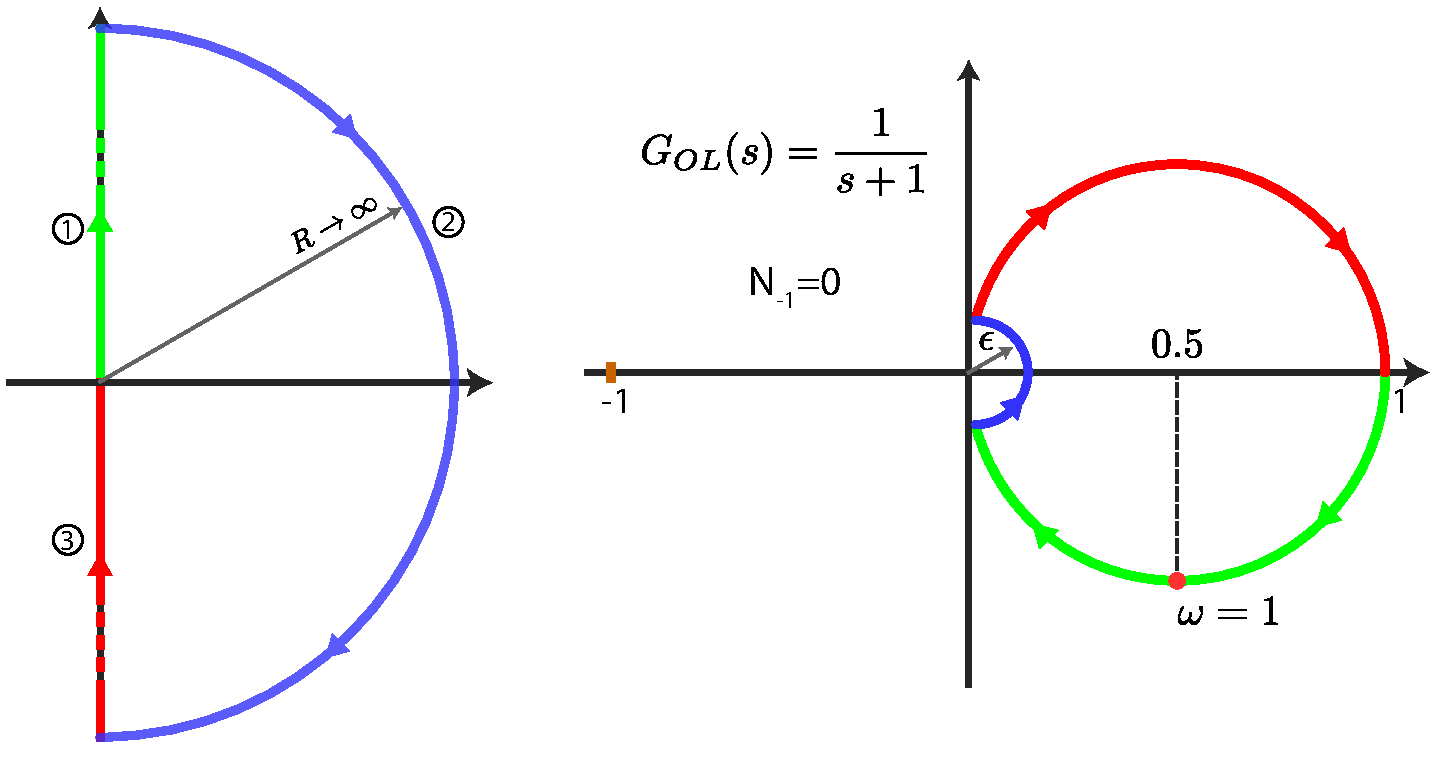
\includegraphics[width=0.9\textwidth]{ex1}
    \end{center}
  \end{minipage}

\vspace{6 pt}

We can conclude from the derived Nyquist plot and
open-loop transfer function

\begin{itemize}
 \item $N = 0$
 \item $P_{OL} = 0$ (since there is no open-loop unstable pole) 
 \item Finally compute $P_{CL} = 0 = \#$ unstable closed-loop poles.
\end{itemize}

Thus the closed-loop system is indeed stable.

\newpage

\subsection{Nyquist Stability for Feedback Systems with Varying DC
Gains}

Now let's consider the following feedback system topology for a SISO
system where DC gain of the open-loop transfer function is adjusted
with a gain parameter $K$ (e.g. P controller). 

\vspace{6 pt}

  \begin{minipage}[h]{1\linewidth}
    \begin{center}
      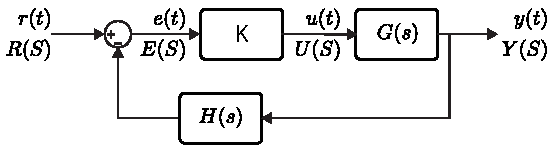
\includegraphics[width=0.5\textwidth]{P}
    \end{center}
  \end{minipage}

\vspace{6 pt}

We would like to test the stability of the closed-loop system
for different values of $K$, moreover we would like to derive 
the range of $K$ values that makes the closed-loop system 
stable. Indeed, we don't need to re-draw the Nyquist plot
for each $K$ that we want to test. 


The analytic function, $F(s)$, that we adopt for analyzing stability 
can be written in the form  
%
\begin{align*}
  F(s) = 1 + G_{OL}(s) = 1 + K \frac{ N(s) }{ D(s) } 
\end{align*}
%
where 
 %
\begin{itemize}
  \item Roots of $N(s)$ are open-loop zeros
  \item Roots of $D(s)$ are open-loop poles
  \item Varible gain parameter $K$
\end{itemize}
%
In order to analyze the stability of Nyquist plot,
in the previous section we showed that 
we can draw the Nyqist plot $G_{OL}(s)$
and analyze the $\#$ encirclements of $(-1 + 0 j)$.

Now, in this case we will derive the Nyquist plot of 
$\frac{N(s)}{D(s)}$, i.e. $\Gamma_{\frac{N(s)}{D(s)}}$. 
Note that $\Gamma_{G_{OL}(s)} = K \Gamma_{\frac{N(s)}{D(s)}}$,
i.e. we simply scale the Nyquist plot of $\frac{N(s)}{D(s)}$
with K (which can be either positive or negative) to find the
Nyquist plot of $G_{OL}(s)$. It is very straightforward to
conclude that 

\vspace{6 pt}

$N \ = \ \#$ of CW enrichments of $(-1 + 0 j)$ by  $\Gamma_{G_{OL}(s)} \
= \ \#$ of CW enrichments of $\left( -\frac{1}{K} + 0 j \right)$ by  $\frac{N(s)}{D(s)}$.

\vspace{6 pt}

To sum-up, in order to analyze the closed-loop stability of a 
feedback systems for which we have a variable gain parameter $K$ in
the open-loop transfer function, we apply the following 
procedure 

\begin{itemize}
 \item Draw the Nyquist plot of $\frac{N(s)}{D(s)}$ where $G_{OL}(s) =
   K \frac{N(s)}{D(s)}$
 \item Compute $N = \ \#$ CW encirclements of $\left( -\frac{1}{K}  + 0 j \right)$ by
   $\Gamma_{ \frac{N(s)}{D(s)} }$ 
 \item Compute $P_{OL} = \ \#$ open-loop poles with
   positive real parts, i.e. $\#$ roots of $D(s)$.
 \item Finally compute $P_{CL} = N +  P_{OL} = \ \#$
   unstable closed-loop poles  
\end{itemize}


\newpage

\textbf{Ex:} Find the range of $K$ values that makes the following
closed-loop system stable.

\vspace{6 pt}

  \begin{minipage}[h]{1\linewidth}
    \begin{center}
      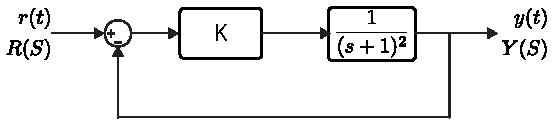
\includegraphics[width=0.45\textwidth]{ex2block}
    \end{center}
  \end{minipage}

\vspace{6 pt}

\textbf{Solution:} For this given system $\frac{N(s)}{D(s)} = \frac{1}{(s+1)^2}$.
In the previous lecture we already derived the Nyquist plot for $\frac{1}{(s+1)^2}$
which is illustrated below

\vspace{6 pt}

  \begin{minipage}[h]{1\linewidth}
    \begin{center}
      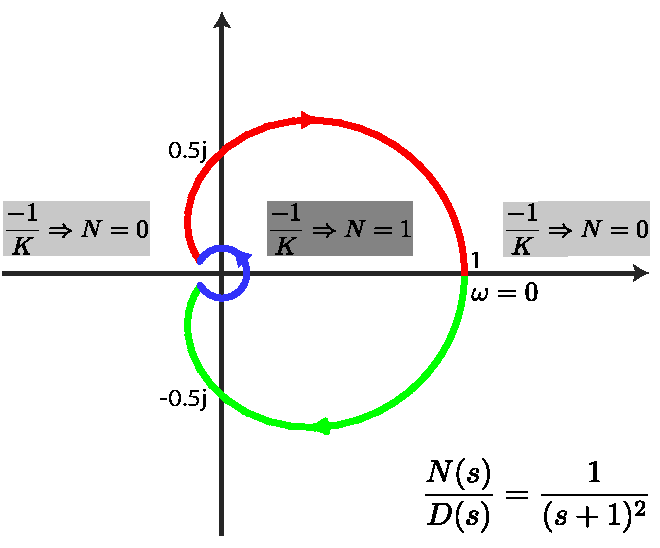
\includegraphics[width=0.57\textwidth]{ex2}
    \end{center}
  \end{minipage}

\vspace{6 pt}

We can see from the derived Nyquist plot that the closed
path divides the real axis in three different parts. If we analyze 
these regions separately, we can then find a complete range of
K values that makes the closed loop-system stable
%
\begin{align*}
  \frac{-1}{K} \in (-\infty ,  0) \ \rightarrow \ K \in [0 , \infty) &\Rightarrow N = 0
  \\
   \frac{-1}{K} \in (0,1)  \ \rightarrow \ K \in (-\infty , -1)  &\Rightarrow N = 1
  \\
  \frac{-1}{K} \in (1,\infty) \rightarrow K \in (-1 , 0] &\Rightarrow N = 0
\end{align*}
%
Note that since number of open-loop unstable poles is equal to 0, 
we have $P_{OL} = 0$. Thus, system is BIBO stable if and only if $N = 0$.
Whereas, for the region when $N = 1$, there always exist one unstable pole. 

Note that for $K = -1$, we don't have a conclusion, indeed system 
is BIBO unstable since in this case there exist a pole on the
imaginary axis. As a result 

\begin{align*}
  K \in (-1 , \infty) \Leftrightarrow \mathrm{BIBO-Stable}
\end{align*}

\newpage

\textbf{Ex:} Find the range of $K$ values that makes the
following closed-loop system stable. Also, for the $K$ values that 
makes the closed-loop system unstable find the number of unstable poles.

\vspace{6 pt}

  \begin{minipage}[h]{1\linewidth}
    \begin{center}
      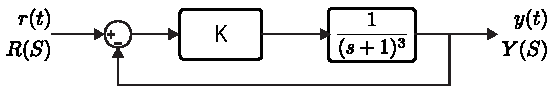
\includegraphics[width=0.5\textwidth]{ex3block}
    \end{center}
  \end{minipage}

\vspace{6 pt}

\textbf{Solution:} For this given system $\frac{N(s)}{D(s)} =
\frac{1}{(s+1)^3}$. In the previous lecture we already derived the
Nyquist plot for $\frac{1}{(s+1)^2}$ which is illustrated below

\vspace{6 pt}

  \begin{minipage}[h]{1\linewidth}
    \begin{center}
      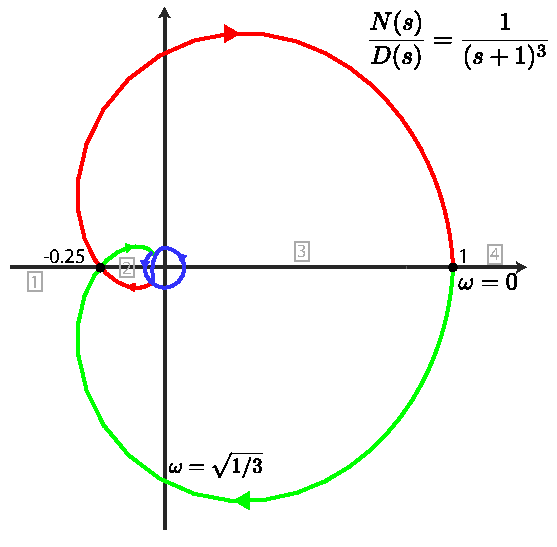
\includegraphics[width=0.6\textwidth]{ex3}
    \end{center}
  \end{minipage}

\vspace{6 pt}

As we can see from the Nyquist plot pf $\frac{1}{(s+1)^3}$, 
it divides the region into four different parts. If we analyze 
these regions separately, we can then find a complete range of
K values that makes the closed loop-system stable, as well as find the
number of unstable poles for the unstable cases. 
%
\begin{enumerate}
  \item $\frac{-1}{K} \in \left( -\infty , \frac{-1}{4} \right) \
    \rightarrow K \in [0 , 4) \ \Rightarrow ( N = 0 , P_{CL} = 0)$, closed-loop system is stable
%
  \item $ \frac{-1}{K} \in \left( \frac{-1}{4} , 0 \right) \
    \rightarrow \ K \in (4, \infty ) \
    \Rightarrow (N = 2 , P_{CL} = 2)$. Unstable CL system
    with 2 unstable poles
%
    \item $ \frac{-1}{K} \in (0 , 1) \ \rightarrow \ K \in (-\infty , -1)    
\Rightarrow (N = 1 , P_{CL} = 1)$. Unstable CL system
    with 1 unstable pole
%
  \item $\frac{-1}{K} \in (1 , \infty) \ \rightarrow \ K \in (-1,0) 
    \Rightarrow ( N = 0 , P_{CL} = 0)$, closed-loop system is stable
\end{enumerate}

As a result 

\begin{align*}
  K \in (-1 , 4 ) \Leftrightarrow \mathrm{BIBO-Stable}
\end{align*}

\newpage

\textbf{Ex:} Find the range of $K$ values that makes the
following closed-loop system stable. Also, for the $K$ values that 
makes the closed-loop system unstable find the number of unstable poles.

\vspace{6 pt}

  \begin{minipage}[h]{1\linewidth}
    \begin{center}
      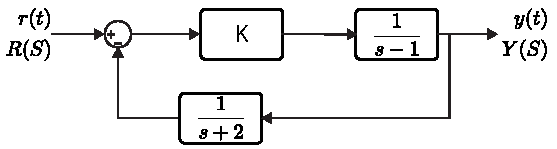
\includegraphics[width=0.5\textwidth]{ex4block}
    \end{center}
  \end{minipage}

\vspace{6 pt}

\textbf{Solution:} For this given system $\frac{N(s)}{D(s)} =
\frac{1}{(s-1)(s+2) }$. Note that for this system $P_{OL} = 1$. 

In the previous lecture we already derived the
Nyquist plot for $\frac{1}{(s-1)(s+2) }$ which is illustrated below

\vspace{6 pt}

  \begin{minipage}[h]{1\linewidth}
    \begin{center}
      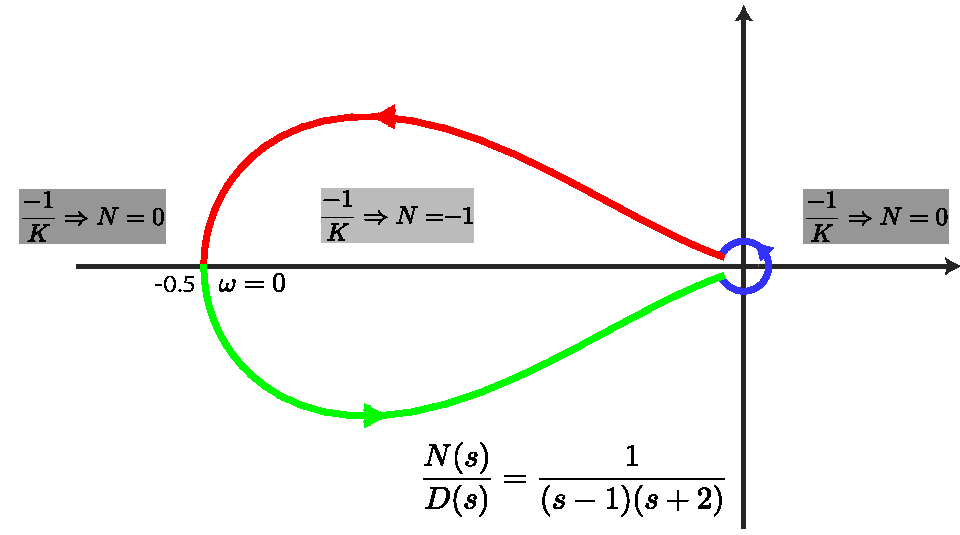
\includegraphics[width=0.75\textwidth]{ex4}
    \end{center}
  \end{minipage}

\vspace{6 pt}

We can see that the Nyquist plot divides the real axis in
three different parts. If we analyze 
these regions separately, we can then find a complete range of
K values that makes the closed loop-system stable
%
\begin{enumerate}
  \item $\frac{-1}{K} \in (-\infty , \frac{-1}{2} ) \ \rightarrow K
    \in (0 , 2) \  \Rightarrow N = 0 \rightarrow P_{CL} = 1$. 
    Unstable CL-system with 1 unstable pole. 
  \item $\frac{-1}{K} \in \left( \frac{-1}{2} , 0 \right) \rightarrow K \in (2 , \infty)  
    \Rightarrow \ N = -1 \rightarrow P = 1 - 1 = 0$. Stable CL-system
  \item $\frac{-1}{K} \in (0 , \infty) \rightarrow K in (-\infty , 0) \Rightarrow N = 0
   \rightarrow P = 1$. Unstable CL-system with 1 unstable pole.
\end{enumerate}
%
As a result 

\begin{align*}
  K \in (2 , \infty) \Leftrightarrow \mathrm{BIBO-Stable}
\end{align*}

\newpage

\subsection{Nyquist Plot and Stability Test with  Open-Loop Poles/Zeros on the Imaginary Axis}

If you remember, when we introduced Nyquist contour and Nyquist stability
test we assumed that there is no pole/zero on the imaginary axis. 
However, it is especially very common to have poles at the origin
since it corresponds to simple integrator. In this course, we will
explicitly cover the case when there exist a pole or zero at the
origin. 

Let's assume that $G_{OL}(s)$ has a pole (or zero, or multiple poles)
at the origin. We simply modify the Nyquist contour by adding an
infinitesimal notch at the origin to the original Nyquist contour. 

The figure below illustrates this modified Nyquist contour and 
an illustrative Nyquist plot. 

\vspace{12 pt}

  \begin{minipage}[h]{1\linewidth}
    \begin{center}
      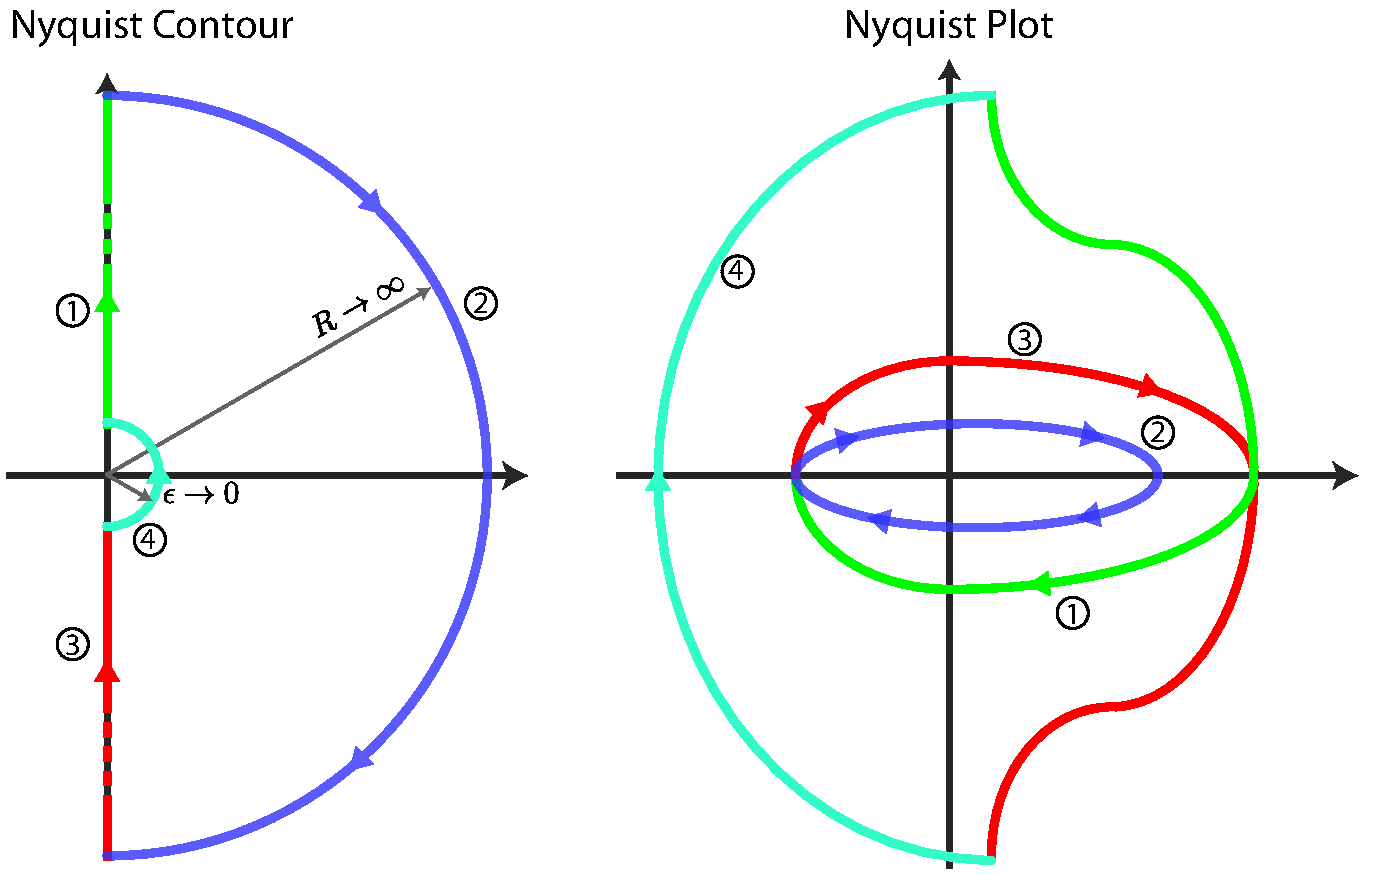
\includegraphics[width=0.8\textwidth]{originnyq}
    \end{center}
  \end{minipage}

\vspace{6 pt}

\newpage

\textbf{Ex:} Find the range of $K$ values that makes the
following closed-loop system stable. 

\vspace{12 pt}

  \begin{minipage}[h]{1\linewidth}
    \begin{center}
      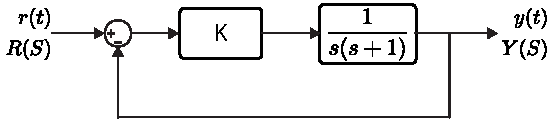
\includegraphics[width=0.65\textwidth]{ex5block}
    \end{center}
  \end{minipage}

\vspace{12 pt}

\textbf{Solution:} For this given system, $\frac{N(s)}{D(s)} =
\frac{1}{s (s+1) }$. Note, there exist a pole at the origin, thus 
we need to utilize the modified Nyquist Contour. 
In the modified Nyquist contour there exist 4 major paths, 
and we need to draw the Nyquist plot based on these 4 paths. 

\begin{enumerate}
  \item This is the polar plot, where we need to plot $G(j \omega)$, where $\omega : 0 \to
    \infty$. 
    % 
    \begin{align*}
      G(j \omega) = \frac{1}{j \omega (j \omega +1)} = \frac{ -j  - \omega }{\omega
      (\omega^2 + 1) } = \frac{-1}{\omega^2 + 1} + \frac{-1/\omega}{
      \omega^2 + 1} j
    \end{align*}
%
   Some observations about polar plot
    \begin{align*}
       Re \lbrace G(j \omega) \rbrace < 0 \quad & \&  \quad  Im \lbrace G(j
                                                \omega) \rbrace < 0 \quad , \ \forall  \omega > 0 
      \\
        \lim_{\omega \to 0} Re \lbrace G(j \omega) \rbrace = - 1
       \quad & \& \quad
       \lim_{\omega \to 0} Re \lbrace G(j \omega) \rbrace = - \infty
        \\
       \lim_{\omega \to \infty} | G(j \omega) | = 0
        \quad & \& \quad
      \lim_{\omega \to \infty} \angle [ G(j \omega) ] = -\pi
      \end{align*}
 %
  \item Note that since we are now only intersted in the circulation around
    $-1/K$. The origin in the Nyquist plot corresponds to $| K | \to
    \infty$, so that it is really not critical to correctly draw this
    detail for feedback systems. 
     However, let's draw this detail for this example for practice. 
     $s = R e^{j \theta}$ and $\theta : \pi/2 \to -\pi/2$.  Then 
   we can derive that  
   \begin{align*}
     & G \left( R e^{j \theta} \right) \approx \frac{1}{R^2 e^{j
       2 \theta}} = \frac{e^{j (-2 \theta)}}{R^2}
       \\
    &\Rightarrow | G \left( R e^{j \theta} \right) | \approx
      \epsilon^2 \ll 1
   \quad , \quad \angle [ G \left( R e^{j \theta} \right) ] \approx -2
      \theta
   \end{align*}
   % 
   Note that when $\theta : \pi/2 \to -\pi/$, the infinite-small 
   contour around origin rotates in CCW direction. 
   %
   \item This part is simply the conjugate of polar plot with reverse
     direction. 
  \item Now this part is new, since we are dealing with this path
    since there is a pole at the origin. 
     $s = \epsilon e^{j \phi}$, where $\epsilon \to 0$ and $\phi :
     -\pi/2 \to \pi/2$ (CCW direction).  Then  we can derive that  
   \begin{align*}
     & G \left( \epsilon e^{j \phi} \right) \approx \frac{1}{\epsilon e^{j
        \phi}} = R e^{j (-\phi)}
       \\
    &\Rightarrow | G \left(\epsilon e^{j \phi} \right) | \approx
     R \ll 1
   \quad , \quad \angle [ G \left( \epsilon e^{j \phi} \right) ] \approx -\phi
   \end{align*}
\end{enumerate}

As a result, we obtain the following Nyquist plot for
$\frac{N(s)}{D(s)} = \frac{1}{s (s+1)}$

\vspace{6 pt}

  \begin{minipage}[h]{1\linewidth}
    \begin{center}
      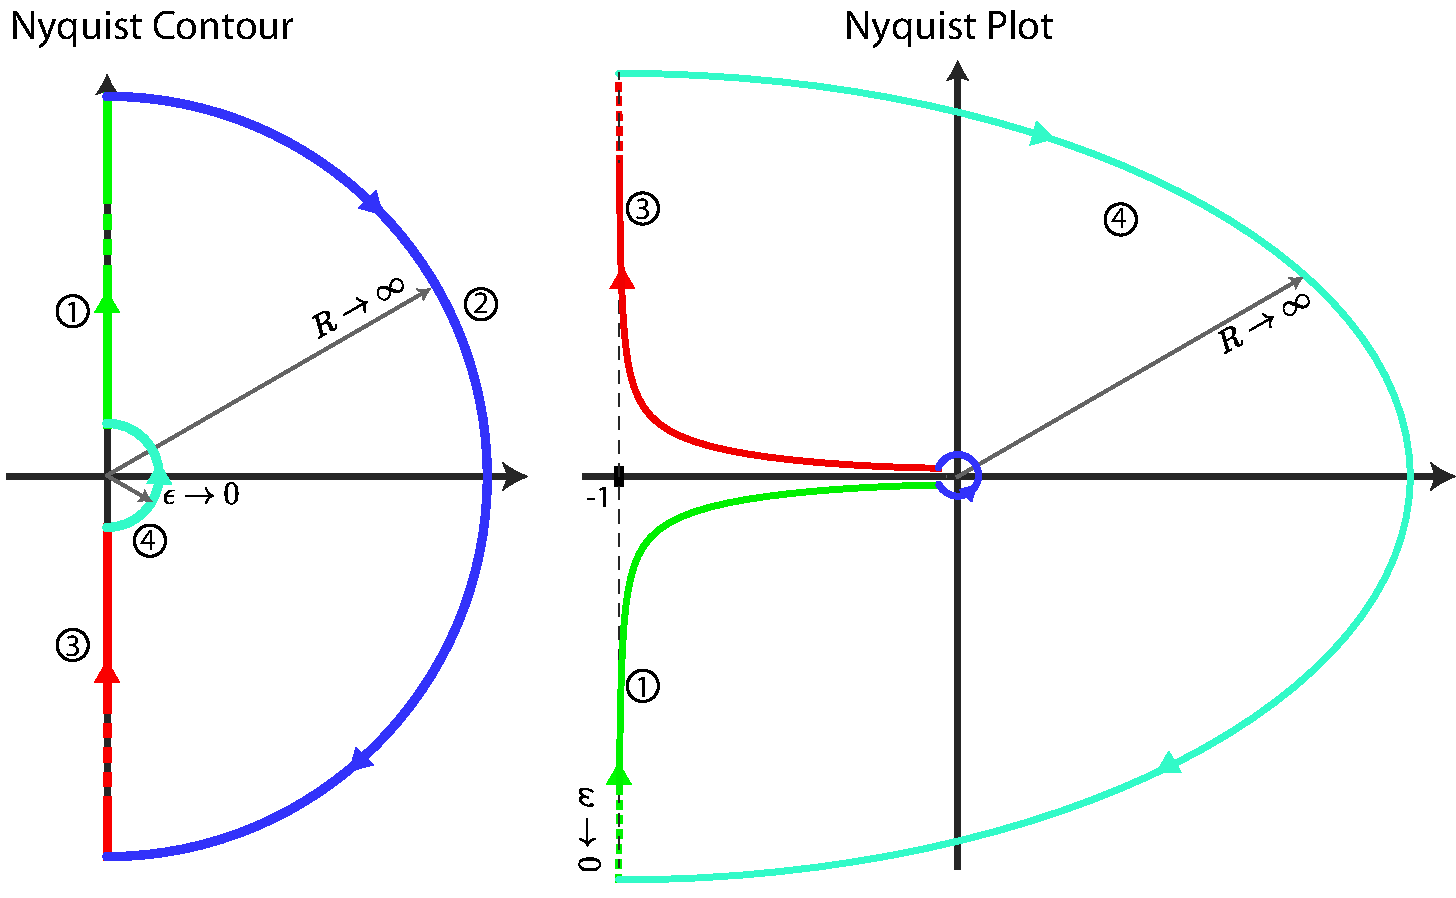
\includegraphics[width=0.85\textwidth]{ex5}
    \end{center}
  \end{minipage}

\vspace{6 pt}

Note that the open-loop transfer function has no unstable poles,
i.e. $P_{OL} = 0$. 
We can see from the Nyquist plot divides the real axis in
two different parts. If we analyze  these regions separately, we can 
then find a range of K values that makes the closed loop-system stable
%
\begin{enumerate}
  \item $\frac{-1}{K} \in (-\infty , 0) \ \rightarrow \ K \in (0 , \infty) 
    \Rightarrow N = 0 \rightarrow P_{CL} = 0 $. System is stable 
  \item $\frac{-1}{K} \in (0, \infty) \rightarrow K \in (-\infty , 0)    
    \Rightarrow N = 1 \rightarrow P_{CL} = 1 $. Unstable system with 1
    unstable pole
\end{enumerate}
%
As a result, $K \in (0 , \infty) \Leftrightarrow $ BIBO-Stable

\newpage

\textbf{Ex:} Find the range of $K$ values that makes the
following closed-loop system stable. 

\vspace{6 pt}

  \begin{minipage}[h]{1\linewidth}
    \begin{center}
      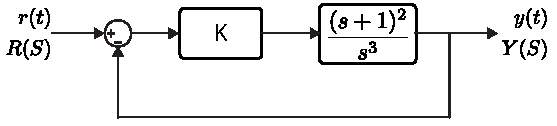
\includegraphics[width=0.5\textwidth]{ex6block}
    \end{center}
  \end{minipage}

\vspace{6 pt}

\textbf{Solution:} For this given system, $\frac{N(s)}{D(s)} =
\frac{(s+1)^2}{s^3}$. Note, there exist three repeated pole at the origin, thus 
we need to utilize the modified Nyquist Contour. 

In the modified Nyquist contour there exist 4 major paths, 
and this we need to draw Nyquist plot based on these 4 paths. 

\begin{enumerate}
  \item This is the polar plot, where we need to plot $G(j \omega)$, where $\omega : 0 \to
    \infty$. 
    % 
    \begin{align*}
      G(j \omega) = \frac{(j\omega + 1)^2 }{(j \omega)^3} 
      = \frac{ (1 - \omega^2) + 2 \omega j}{ -j \omega^3}
     = \frac{ (1 - \omega^2) j - 2 \omega}{\omega^3}
       = \frac{- 2 }{\omega^2} + \frac{ 1 - \omega^2 }{\omega^3} j
    \end{align*}
%
   Some observations about polar plot
    \begin{align*}
       Re \lbrace G(j \omega) \rbrace < 0 
      \\ 
       Im \lbrace G(j \omega) \rbrace > 0 \quad , \ \forall  \omega \ \in
      (0, 1) 
      \\
       Im \lbrace G(j \omega) \rbrace < 0 \quad , \ \forall  \omega \ \in
      (1,\infty) 
      \\
      [ G(j \omega) ]_{\omega = 1} = -2 + 0 j
      \\
        \lim_{\omega \to 0}  | G(j \omega)  | = \infty
       \quad & \& \quad
       \lim_{\omega \to 0} \angle [ G(j \omega) ] = \pi/2  
        \\
       \lim_{\omega \to \infty} | G(j \omega) | = 0
        \quad & \& \quad
      \lim_{\omega \to \infty} \angle [ G(j \omega) ] = -\pi/2
      \end{align*}
 %
  \item Note that since we are intersted in the circulation around
    $-1/K$ and origin in the Nyquist plot corresponds to $| K | \to
    \infty$, it is really not critical to correctly draw this detail. 
    Thus we will omit it for this problem.
   %
   \item This part is simply the conjugate of polar plot with reverse
     direction. 
  \item This part is very critical for stability analysis
     $s = \epsilon e^{j \phi}$, where $\epsilon \to 0$ and $\phi :
     -\pi/2 \to \pi/2$ (CCW direction).  Then  we can derive that  
   \begin{align*}
     & G \left( \epsilon e^{j \phi} \right) \approx \frac{1}{\epsilon^3 e^{j
        3\phi}} = R^3 e^{j (-3 \phi)}
       \\
    &\Rightarrow | G \left(\epsilon \ e^{j \phi} \right) | \approx
     R^3 \to \infty 
   \quad , \quad \angle [ G \left( \epsilon \ e^{j \phi} \right) ]
      \approx -3 \phi
   \end{align*}
  Note that this path is a 1.5 circle that turns in CW direction
\end{enumerate}

As a result, we obtain the following Nyquist plot for
$\frac{N(s)}{D(s)} = \frac{(s+1)^2}{s^3}$

\vspace{6 pt}

  \begin{minipage}[h]{1\linewidth}
    \begin{center}
      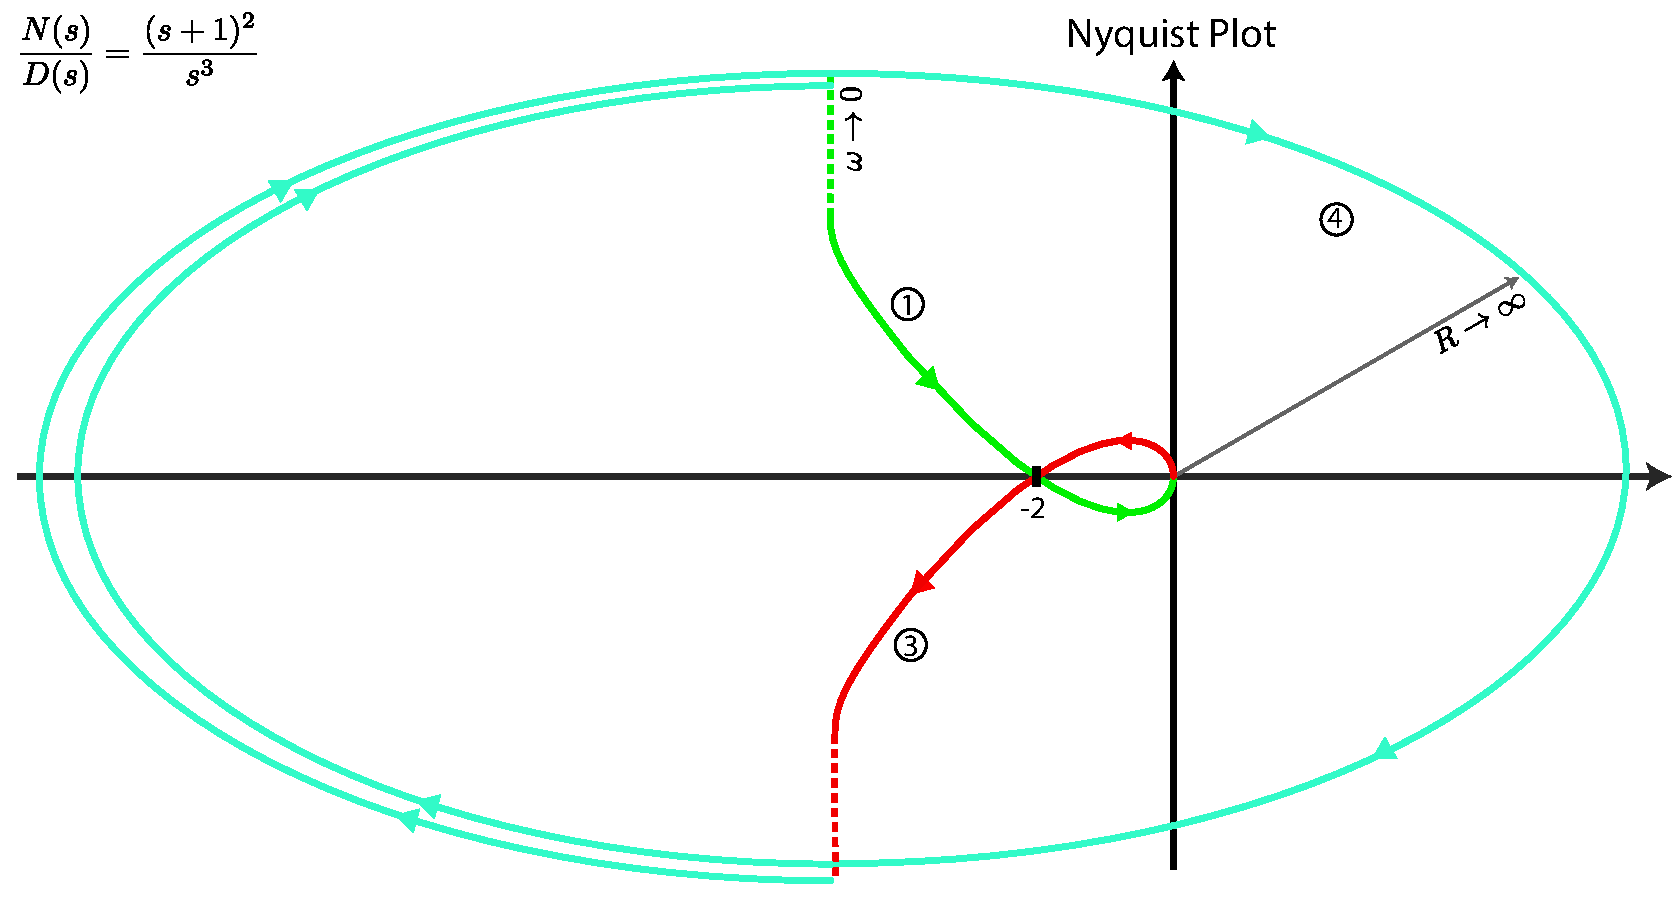
\includegraphics[width=0.8\textwidth]{ex6}
    \end{center}
  \end{minipage}

\vspace{6 pt}

Note that the open-loop transfer function has no unstable poles,
thus $P_{OL} = 0$. We can see that the derived Nyquist plot divides the real axis in
three different parts. If we analyze  these regions separately, we can 
then find a range of K values that makes the closed loop-system stable
%
\begin{enumerate}
  \item $\frac{-1}{K} \in (-\infty , - 2) \rightarrow K \in (0 , 2) \Rightarrow N = 2 \rightarrow P_{CL} = 2 $. Unstable system with
    2 unstable poles. 
  \item $\frac{-1}{K} \in (-2 , 0) \rightarrow K \in (2 , \infty)
    \Rightarrow N = 0 \rightarrow P_{CL} = 0 $. System is stable
    \item $\frac{-1}{K} \in (0,\infty) \rightarrow K \in (-\infty , 0)
    \Rightarrow N = 1 \rightarrow P_{CL} = 1 $. Unstable system with
    1 unstable pole. 
\end{enumerate}
%
As a result, $K \in (2 , \infty) \Leftrightarrow $ BIBO-Stable


% **** This ENDS THE EXAMPLES. DON'T DELETE THE FOLLOWING LINE:
\end{document}